\documentclass[oneside, letterpaper, 10pt, oldfontcommands]{memoir}
\usepackage{uwthesis}

%\usepackage[caption=false]{subfig}
%\usepackage{subfigure}
\usepackage{graphicx}
\usepackage{bm}
\usepackage{amssymb}
\usepackage{amsmath}
\usepackage{amsfonts}
\usepackage[utf8]{inputenc}
\usepackage{placeins}
% defines table rules for professional looking tables
\usepackage{booktabs}
\usepackage{gensymb}
\usepackage[colorlinks=true,allcolors=blue]{hyperref}
\usepackage{microtype}
\usepackage{multirow, makecell}
\usepackage[capitalise]{cleveref}
\usepackage[utf8]{inputenc}
\usepackage[T5,T1]{fontenc}
\usepackage{listings}
\usepackage{siunitx}
%\sisetup{detect-weight=true, detect-family=true}
\sisetup{detect-all = true}
\usepackage{xspace}
\usepackage{comment}
\usepackage{ragged2e}
\usepackage{lineno}
\usepackage{subfiles}
\usepackage{textcomp}
\usepackage{rotating}
\usepackage{subcaption}
\usepackage{longtable}
\usepackage[compat=1.1.0]{tikz-feynman}
\usepackage{multicol}
\usepackage[bibstyle=ieee,citestyle=numeric,sorting=none]{biblatex}

\newcommand{\Python}{\texttt{Python}}
\newcommand{\MCEq}{\texttt{MCE{\scriptsize Q}}}
\newcommand{\MMC}{\texttt{MMC}}
\newcommand{\PROPOSAL}{\texttt{PROPOSAL}}
\newcommand{\CORSIKA}{\texttt{CORSIKA}}
\newcommand{\MUONGUN}{\texttt{MUONGUN}}
\newcommand{\PHOTOSPLINE}{\texttt{PHOTOSPLINE}}
\newcommand{\like}{\mathcal{L}}
\newcommand{\likeSAY}{\mathcal{L}_{\textrm{Eff}}}
\newcommand{\pdfSxi}{S(\vec{x}_i)}
\newcommand{\TS}{\mathrm{TS}}
\newcommand{\Fermi}{\textit{Fermi}}
\newcommand{\nuveto}{{\LARGE $\nu$}\texttt{eto}}

\DeclareMathOperator*{\argmax}{arg\,max}
\DeclareMathOperator*{\argmin}{arg\,min}

\newcommand{\refeq}[1]{Eq.~(\ref{#1})}
\newcommand{\refeqs}[2]{Eqs.~(\ref{#1})~and~(\ref{#2})}
\newcommand{\refeqss}[3]{Eqs.~(\ref{#1}), (\ref{#2})~and~(\ref{#3})}
\newcommand{\reffig}[1]{Fig.~\ref{#1}}
\newcommand{\reffigs}[2]{Figs.~\ref{#1}~and~\ref{#2}}
\newcommand{\refsec}[1]{Section~\ref{#1}}
\newcommand{\refsecs}[5]{Sections~\ref{#1},~\ref{#2},~\ref{#3},~\ref{#4},~and~\ref{#5}}
\newcommand{\refappsec}[1]{Appendix Section~\ref{#1}}
\newcommand{\refapp}[1]{Appendix~\ref{#1}}
\newcommand{\reftab}[1]{Table~\ref{#1}}
\newcommand{\refref}[1]{Ref.~\cite{#1}}
\newcommand{\refrefs}[2]{Refs.~\cite{#1}~and~\cite{#2}}

\newcommand{\vectheta}{\vec{\theta}}
\newcommand{\vecw}{\vec{w}}
\newcommand{\prob}{\mathcal{P}}
\newcommand{\gprob}{\mathcal{G}}
\newcommand{\meanl}{\mathcal{L}_{\textmd{Mean}}}
\newcommand{\mcl}{\like_\textmd{Eff}}
\newcommand{\gl}{\like_\textmd{G}}
\newcommand{\adhoc}{\mathcal{L}_{\textmd{AdHoc}}}
\newcommand{\lpoisson}{l_{\textmd{Poisson}}}
\newcommand{\lmc}{l_\textmd{Eff}}
\newcommand{\lbarlow}{\like_{\textmd{BB}}}
\newcommand{\hatmu}{\hat{\mu}}
\newcommand{\hatpoisson}{\hatmu_\textmd{Poisson}}
\newcommand{\hatmc}{\hatmu_\textmd{Eff}}
\newcommand{\au}{arb. unit}
\newcommand{\agpar}{\alpha}
\newcommand{\bgpar}{\beta}
\newcommand{\emcee}{\texttt{emcee}}
\newcommand{\meff}{m_\mathrm{Eff}}
\newcommand{\weff}{w_\mathrm{Eff}}
\newcommand{\superk}{Super--Kamiokande\xspace}

\newcommand{\Emf}{E_{\mu}^{\rm f}}
\newcommand{\Emi}{E_{\mu}^{\rm i}}
\newcommand{\ECR}{E_{\rm CR}}
\newcommand{\Prob}{{\cal P}}
\newcommand{\Ppuncor}{\Prob_{\rm pass}^{\rm uncor}}
\newcommand{\Ppcor}{\Prob_{\rm pass}^{\rm cor}}
\newcommand{\Pzmproto}{\Prob_{0\mu}^{\rm shower}}
\newcommand{\Pzmsib}{\Prob_{0\mu}^{\rm sib}}
\newcommand{\Pzm}{\Prob_{0\mu}}
\newcommand{\barparen}[2]{\overset{\scriptscriptstyle (-)}{#1}_{\!\!#2}}

% This holds definitions of macros to enforce consistency in units.

% This file is the sole location for such definitions.  Check here to
% learn what there is and add new ones only here.

% also see defs.tex for names.


% see
%  http://ctan.org/pkg/siunitx
%  http://mirrors.ctan.org/macros/latex/contrib/siunitx/siunitx.pdf

% Examples:
%  % angles
%  \ang{1.5} off-axis
%
%  % just a unit
%  \si{\kilo\tonne}
%
%  % with a value:
%  \SI{10}{\mega\electronvolt}

%  range of values:
% \SIrange{60}{120}{\GeV}

% some shorthand notation
%\DeclareSIUnit \MBq {\mega\Bq}
\DeclareSIUnit \s {\second}
\DeclareSIUnit \ns {\nano\second}
\DeclareSIUnit \mus {\micro\second}
\DeclareSIUnit \ms {\milli\second}
\DeclareSIUnit \MB {\mega\byte}
\DeclareSIUnit \GB {\giga\byte}
\DeclareSIUnit \TB {\tera\byte}
\DeclareSIUnit \PB {\peta\byte}
\DeclareSIUnit \Mbps {\mega\bit/\s}
\DeclareSIUnit \Gbps {\giga\bit/\s}
\DeclareSIUnit \Tbps {\tera\bit/\s}
\DeclareSIUnit \Pbps {\peta\bit/\s}
\DeclareSIUnit \kton {\kilo\tonne} % changed  back to kton
\DeclareSIUnit \kt {\kilo\tonne}
\DeclareSIUnit \Mt {\mega\tonne}
\DeclareSIUnit \eV {\electronvolt}
\DeclareSIUnit \keV {\kilo\electronvolt}
\DeclareSIUnit \MeV {\mega\electronvolt}
\DeclareSIUnit \GeV {\giga\electronvolt}
\DeclareSIUnit \PeV {\peta\electronvolt}
\DeclareSIUnit \EeV {\exa\electronvolt}
\DeclareSIUnit \m {\meter}
\DeclareSIUnit \cm {\centi\meter}
\DeclareSIUnit \in {\inchcommand}
\DeclareSIUnit \km {\kilo\meter}
\DeclareSIUnit \kV {\kilo\volt}
\DeclareSIUnit \kW {\kilo\watt}
\DeclareSIUnit \MW {\mega\watt}
\DeclareSIUnit \MHz {\mega\hertz}
\DeclareSIUnit \mrad {\milli\radian}
\DeclareSIUnit \year {years}
\DeclareSIUnit \POT {POT}
\DeclareSIUnit \sig {$\sigma$}
\DeclareSIUnit\parsec{pc}
\DeclareSIUnit\lightyear{ly}
\DeclareSIUnit\foot{ft}
\DeclareSIUnit\ft{ft}
\DeclareSIUnit \ppb{ppb}
\DeclareSIUnit \ppt{ppt}
\DeclareSIUnit \samples{S}
\DeclareSIUnit \pe{PE}
\DeclareSIUnit \sr{\steradian}

\newcommand\SigmaOne{\SI{68.3}\percent}
\newcommand\SigmaTwo{\SI{95.4}\percent}

% "the Glashow Resonance energy"
\newcommand\GlashowEnergy{\SI{6.3}\PeV\xspace}
%

% The reconstructed deposited energy cut
\newcommand\EnergyCut{\SI{60}\TeV\xspace}

% The sample livetime
\newcommand\Livetime{\SI{7.5}\year\xspace}

% The segmented power law
\newcommand\minunfoldingenergy{1.995\times10^4}
\newcommand\maxunfoldingenergy{3.162\times10^8}
\newcommand\unfoldingsegments{13}

% Analysis parameters
\newcommand\astronorm{\Phi_\texttt{astro}}
\newcommand\astrodeltagamma{\gamma_\texttt{astro}}
\newcommand\convnorm{\Phi_\texttt{conv}}
\newcommand\promptnorm{\Phi_\texttt{prompt}}
\newcommand\pik{R_{K/\pi}}
\newcommand\atmonunubar{{2\nu/\left(\nu+\bar{\nu}\right)}_\texttt{atmo}}
\newcommand\crdeltagamma{\Delta\gamma_\texttt{CR}}
\newcommand\muonnorm{\Phi_\mu}
\newcommand\domeff{\epsilon_\texttt{DOM}}
\newcommand\holeice{\epsilon_\texttt{head-on}}
\newcommand\anisotropy{a_s}

% Parameters not in the analysis


\chapter{Analysis}\label{chapter:analysis}

The goal of the analysis in this chapter is to characterize the astrophysical neutrino spectrum using a high-purity sample of events.
On its own, this may not provide the great insight that we desire into larger problems of astropysical neutrino origin or cosmic ray acceleration mechanisms.
However, the detailed measurements performed here are a vital piece of the puzzle that may help us to answer these larger questions in the long run.
In pursuit of these measurements a handful of new techniques were also developed, and these will certainly improve the other measurements we make going forward.
This chapter combines the analysis components outlined in previous chapters with different definitions of the astrophysical neutrino flux and applies the statistical inference techniques of \refsec{sec:statistics} to the analysis structure of \reffig{fig:analysis_overview}.
With this a wide variety of tests and measurements of the astrophysical flux are explored and their results examined.

\section{Characterization of the astrophysical neutrino flux\label{sec:diffuse}}
\begingroup
\graphicspath{{results/HESE_Final_Paper/}}
\input{results/HESE_Final_Paper/sections/diffuse/diffuse}
\endgroup

\subsection{Generic models\label{sec:generic_models}}
\begingroup
\graphicspath{{results/HESE_Final_Paper/}}
\input{results/HESE_Final_Paper/sections/diffuse/generic_models}
\endgroup

\subsubsection{Single power-law flux\label{sec:spl}}
\begingroup
\graphicspath{{results/HESE_Final_Paper/}}
\input{results/HESE_Final_Paper/sections/diffuse/spl}
\endgroup

\subsubsection{Double power-law flux\label{sec:dpl}}
\begingroup
\graphicspath{{results/HESE_Final_Paper/}}
\input{results/HESE_Final_Paper/sections/diffuse/dpl}
\endgroup

\subsubsection{Single power law with spectral cutoff\label{sec:cutoff}}
\begingroup
\graphicspath{{results/HESE_Final_Paper/}}
\input{results/HESE_Final_Paper/sections/diffuse/cutoff}
\endgroup

\subsubsection{Log-parabola flux\label{sec:log_parabola}}
\begingroup
\graphicspath{{results/HESE_Final_Paper/}}
\input{results/HESE_Final_Paper/sections/diffuse/lppl}
\endgroup

\subsubsection{Segmented power-law flux\label{sec:unfolding}}
\begingroup
\graphicspath{{results/HESE_Final_Paper/}}
\input{results/HESE_Final_Paper/sections/diffuse/segmented}
\endgroup

\subsection{Atmospheric flux from charmed hadrons\label{sec:prompt}}
\begingroup
\graphicspath{{results/HESE_Final_Paper/}}
\input{results/HESE_Final_Paper/sections/diffuse/prompt}
\endgroup

\subsection{Source-specific models\label{sec:specific_models}}
\begingroup
\graphicspath{{results/HESE_Final_Paper/}}
\input{results/HESE_Final_Paper/sections/diffuse/specific_models}
\endgroup
\input{results/mcllh_paper/tex/mc_diagram_preamble}

\settitle{Precision measurements of the astrophysical neutrino flux}
\setauthor{Austin Schneider}
\setdepartment{Physics}
\doctors
\setgraddate{2020}
\setdefensedate{August 6th 2020}

\setfoca{Keith Bechtol}{Assistant Professor}{Physics}
\setfocb{Jessi Cisewski-Kehe}{Assistant Professor}{Statistics}
\setfocc{Francis L Halzen}{Professor}{Physics}
\setfocd{Albrecht Karle}{Professor}{Physics}

\setabstract{The IceCube neutrino observatory has established the existence of a high-energy all-sky neutrino flux of astrophysical origin.
	This discovery was made using events interacting within a fiducial region of the detector surrounded by an active veto with reconstructed energy above \EnergyCut, commonly known as the high-energy starting event sample or HESE\@.
	We revisit the analysis of the HESE sample with an additional $\SI{4.5}\year$ of data, newer glacial ice models, and improved systematics treatment.
	This paper gives a detailed description of the sample, reports on the latest astrophysical neutrino flux measurements, and presents a source search for astrophysical neutrinos.
	We give the compatibility of these observations with specific isotropic flux models proposed in the literature as well as generic power-law-like scenarios.
	We find that the astrophysical neutrino spectrum, when assumed equal for neutrinos and anti-neutrinos and among neutrino flavors, is compatible with an unbroken power law, with a preferred spectral index of  $\SPLFreqBFIndex^{+\SPLFreqWilksUpperIndexDelta}_{-\SPLFreqWilksLowerIndexDelta}$ for the $\SigmaOne$ confidence interval.}

%\bibliographystyle{ieeetr}
\addbibresource{results/HESE_Final_Paper/hesebiblio.bib}
\addbibresource{results/mcllh_paper/likelihood.bib}
\addbibresource{results/passing_fractions_paper/nuveto.bib}
\addbibresource{thesis-citations.bib}
\setlrmarginsandblock{1in}{1in}{*}
\setulmarginsandblock{1in}{1in}{*}
\checkandfixthelayout
\setsecnumdepth{paragraph}
\maxtocdepth{subsection}

\linenumbers{}

\begin{document}


\frontmatter

\thetitlepage
\cleardoublepage
\setcounter{page}{1}

%\section{Abstract}
%\uwabstract
%\cleardoublepage

\section{Acknowledgements}

The body of work that follows tells a story of scientific achievement, highlighting the incremental progress others and I have made. However, it neglects something far more important, the people and community behind it all. Unfortunately, I have neither the time nor space to thank everyone properly. I have had incredible support from friends, family, mentors, communities of fellow scientists, among many others throughout this journey. Without their help, support, and constant positive influence, I would not be where I am now, nor would I be the person I am today.

Thank you, Albrecht, for your guidance, light-hearted perspective, and prudent advice. Your persistent input has helped me become a better scientist and communicator, despite my own stubbornness at times. There is still much for me to learn, but I have you to thank for setting me on the right track and keeping me from getting lost in the metaphorical woods. Carlos, Tianlu, Juliana, and Nancy, we've shared a long and challenging road bringing our analyses to fruition. Still, I hope you all remember some of the fun we had along the way. You all pushed me to be better in different ways, and it has been a blast having you as collaborators. I'm fortunate to have been surrounded by the fantastic people at WIPAC. I couldn't ask for a better bunch as friends and colleagues to accompany me through these years. Your attitudes, eagerness, and excitement have been absolutely contagious, and I have been humbled by your generosity and selfless drive to improve the institutions that shape our lives. I hope to see you all in the future, even as we depart from our shared experiences at WIPAC.

To my parents, Margaret and James, thank you for your unconditional love and support. You've been there for me at every turn.

\clearpage
\tableofcontents\clearpage
%\listoffigures\clearpage
%\listoftables\clearpage

\mainmatter
%\linenumbers

\chapter{Introduction}\label{chapter:introduction}

\begingroup
\graphicspath{{results/HESE_Final_Paper/}}
\subfile{results/HESE_Final_Paper/sections/introduction}
\endgroup

\chapter{Background Information}\label{chapter:background}

\section{Neutrino interactions and detection}

Neutrinos are the only neutral leptons in the standard model of particle physics.
Although fundamentally neutrinos only interact through gravity and the exchange of weak bosons, there exist a wide range of processes that dominate the relevant physical behavior of neutrinos at different energy scales.
Such interactions include: nuclear capture, inverse beta-decay, quasi-elastic scattering, resonant particle production, coherent elastic scattering, deep inelastic scattering (DIS), and ultra-high energy interactions~\ref{Vannucci:2017rqs,Akimov:2017ade}.
Above $\si\TeV$ neutrino energies however, only two known processes remain relevant for detection: DIS and resonant $W$ production.
Deep inelastic scattering refers to processes that probe the fundamental components of hadrons.
For neutrinos, this means the exchange of a weak boson with a quark.
The momentum imparted to the quark will produce a hadronic cascade of secondary particles.
The details of the lepton side of the interaction depend heavily on the species of incident neutrino and weak boson exchanged.
We can divide these DIS interactions into two categories based on the weak boson exchanged.
Interactions involving the exchange of a $Z$ are referred to as ``neutral current'' (NC), and those exchanging a $W$ are referred to as ``charged current'' (CC).
Modern techniques for observing neutrino interactions rely on detecting the charged particle products of the initial interaction.
As a consequence of this, the observable energy can be very different for NC and CC events.
Both interactions produce a hadronic cascade, but on the leptonic side of the interaction NC event have an outgoing neutrino (not observable) while CC events have an outgoing charged lepton (observable).
These two interactions are shown in \reffig{fig:DIS}.

\begin{figure}
	\centering
	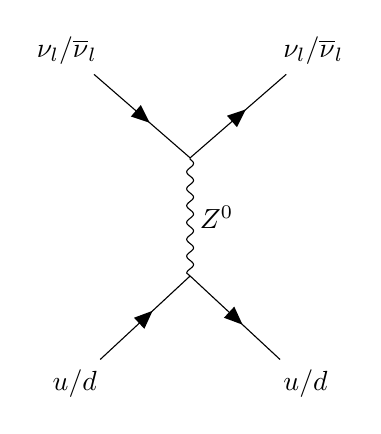
\begin{tikzpicture}
	\begin{feynman}
	\vertex (a);
	\vertex [below=of a] (b);
	\vertex [above left=of a] (c) {\(\nu_{l} / \overline \nu_{l}\)};
	\vertex [above right=of a] (d) {\(\nu_{l} / \overline \nu_{l}\)};
	\vertex [below left=of b] (e) {\(u/d\)};
	\vertex [below right=of b] (f) {\(u/d\)};
	\diagram* {
		(c) -- [fermion] (a),
		(a) -- [fermion] (d),
		(e) -- [fermion] (b),
		(b) -- [fermion] (f),
		(a) -- [boson, edge label=\(Z^0\)] (b),
	};
	\end{feynman}
	\end{tikzpicture}
	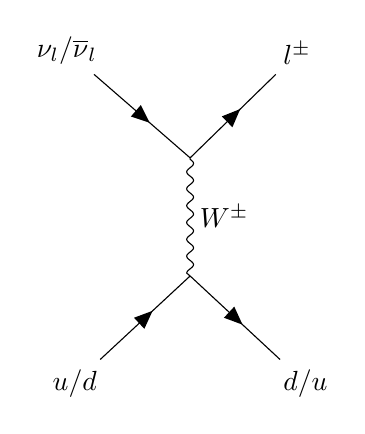
\begin{tikzpicture}
	\begin{feynman}
	\vertex (a);
	\vertex [below=of a] (b);
	\vertex [above left=of a] (c) {\(\nu_{l} / \overline \nu_{l}\)};
	\vertex [above right=of a] (d) {\(l^\pm\)};
	\vertex [below left=of b] (e) {\(u/d\)};
	\vertex [below right=of b] (f) {\(d/u\)};
	\diagram* {
		(c) -- [fermion] (a),
		(a) -- [fermion] (d),
		(e) -- [fermion] (b),
		(b) -- [fermion] (f),
		(a) -- [boson, edge label=\(W^\pm\)] (b),
	};
	\end{feynman}
	\end{tikzpicture}
	\caption{The neutrino deep inelastic scattering processes NC (left) and CC (right) in matter is shown in the figure above for interactions with nucleon component quarks.
	In both cases, significant momentum can be imparted to the outgoing quark which will result in the production of a hadronic particle cascade.
	In NC interactions, only the hadronic cascade may be detectable as the interaction product is a neutrino which is unlikely to undergo another interaction within the detection medium.
	Interactions of the CC variety on the other hand, produce a charged lepton in addition to the hadronic cascade.
	This charged lepton can also be detected if it receives enough energy.}
	\label{fig:DIS}
\end{figure}

The third interaction relevant above $\si\TeV$ neutrino energies is the resonant production of a $W$ boson, otherwise known as the Glashow resonance (GR)~\cite{Glashow:1960zz}.
In matter on Earth this process occurs when an anti-electron neutrino combines with an atomic electron to produce an on-shell $W^+$ as shown in~\reffig{fig:glashow}
If we consider the rest frame of the electron, then this resonance occurs at a neutrino energy of $\SI{6.3}\PeV$.
For atomic electrons we should consider the rest frame of the atom, and in this case there is a Doppler broadening of the resonance of $\sim\SI{20}\percent$ due to the orbital motion of the electrons~\cite{Loewy:2014zva}.
In practice this broadening is small in comparison to the energy resolution of modern neutrino detectors that have access to this energy scale, and any further broadening from thermal motion will be even smaller.
The production of a $W^+$ and it's subsequent decay can result in either a hadronic shower similar to a NC interaction, or a leptonic final state similar to a CC interaction.
These two possibilities correspond to the hadronic and leptonic decay modes of the $W$ respectively.

\begin{figure}
	\centering
	\begin{tikzpicture}
	\begin{feynman}
	\vertex (a);
	\vertex [right=of a] (b);
	\vertex [above left=of a] (c) {\(\overline \nu_{e}\)};
	\vertex [below left=of a] (d) {\(e^-\)};
	\diagram* {
		(c) -- [fermion] (a),
		(a) -- [fermion] (d),
		(a) -- [boson, edge label=\(W^+\)] (b),
	};
	\end{feynman}
	\end{tikzpicture}
	\caption{The production of an on-shell $W^+$ boson through the combination of an anti-electron neutrino and electron.
	This resonant process occurs at neutrino energies around $\SI{6.3}\PeV$.}
	\label{fig:glashow}
\end{figure}

Through either a NC interaction or the hadronic decay of a $W$ boson, neutrinos can induce a hadronic shower.
In a hadronic shower, both charged hadrons and leptons are produced which can be detected through well established methods.
Charged current interactions produce a hadronic shower by imparting momentum to a quark which is then hadronized, although the charged lepton produced in the interaction is also detectable and can significantly alter the detection signature of the event.

Through either a CC interaction or the leptonic decay of a $W$ boson, neutrinos can produce a detectable charged lepton, although the detection signature differs depending on the flavor of charged lepton produced.
Focusing on dense detection media like ice or water, the detection signatures of the three flavor of charged lepton are as follows.
High energy electrons and positrons immediately interact with the detection media to initiate an electromagnetic cascade where charge leptons and high energy photons are alternately produced by one another.
This electromagnetic cascade develops in a roughly spherical fashion within the dense detection medium, but has a directional bias because of the momentum of the first charged lepton.

Muons from high energy neutrino interactions do not interact as readily as electrons and positrons due to their larger mass.
Instead, muons are able to travel several kilometers in dense media before eventually losing enough energy that they quickly decay.
Along their entire path length, muons lose energy by interacting with the detection medium.
These ``energy loss'' interactions include ionization, electron-positron pair production, bremsstrahlung, and photo-nuclear interactions.
Although these processes are highly stochastic, the average energy loss of muons approximately follows $-dE/dx=a+bE$ where $a$ is determined by the ionization energy losses and $b$ is defined by the other processes.
In general $a$ and $b$ and both functions of the muon energy $E$, but this linear approximation where $a$ and $b$ are constant holds locally as both are slowly varying as a function of $E$.
For muon energies above $\SI{1}\TeV$, the so called ``radiative'' term $bE$ dominates the average energy losses.
Thus, the energy loss rate in a detection medium can be used to infer the muon energy.
In practice the muon energy can be determined to within a factor of $2$, however improved techniques may achieve a resolution as small as $\SI{10}\percent$ in the future.

Taus produced similarly are also detectable.
The short decay length of a tau, $\SI{50}\meter / \si\PeV$, means it is likely to decay very close to the neutrino interaction vertex.
Taus decay hadronically with a branching ratio of $\SI{64.79}\percent$, which results in a hadronic shower.
Leptonic decay modes of the tau are decay to a charged lepton and corresponding neutrino of either electron or muon flavor.
In the electron case, an electromagnetic shower results; whereas in the muon case a far travelling muon is produced.
For taus produced via the decay of a $W$ boson, the event is indistinguishable from taus produces via CC and NC interactions other than by resonance energy at which this process occurs, as tau energy losses are negligible in the short decay length.

From the wide variety of methods for detecting charged particles, water Cherenkov detectors are most common for detecting neutrinos in this high-energy regime above $\SI{1}\TeV$.
Water Cherenekov detectors have the advantage that their detection medium is both abundant and inexpensive.
The high-energy charged leptons themselves do not produce many Cherenkov photons.
However, as these leptons lose energy in the detection medium, the secondary particle showers they produce give rise to many Cherenkov photons.
This light yield allows these detectors to be sparsely instrumented while maintaining detection efficiency and reconstruction quality.

Water Cherenkov detectors often make use of photo-multiplier-tubes (PMTs) to detect Cherenkov photons.
PMTs have a thin photo-cathode that is held at a high-voltage differential with respect to an anode; this allows the production and acceleration of a photo-electron when photons pass through the photo-cathode.
Accelerated photo-electrons hurtle towards a an amplification stage composed of many dynodes, each held at a large voltage difference to the adjacent dynodes.
This setup allows a single photo-electron to produce many secondary electrons upon interaction with a dynode, starting an exponential cascade of electrons across the dynode stages.
The resulting cascade of electrons is amplified enough with respect to the original signal that they can be detected electronically as a voltage change.
In this way, PMTs can be sensitive to single photons, provided one is able to reach the photo-cathode.

\section{Cosmic rays and air showers}

\textbf{What are cosmic rays?}

\textbf{How do cosmic rays relate to water Cherenkov detectors?}

\textbf{How do cosmic rays produce muons and neutrinos?}

\textbf{What are the properties of the muon and neutrino fluxes we need to be concerned with?}

Cosmic rays are high-energy protons and atomic nuclei that propagate through space.
Some of these particles originate from our own sun, and within the Milky Way.
However, the highest energy population of cosmic rays has been shown be distinct from the lower energy population and likely of extra-galactic origin.
The sources and acceleration mechanisms of these extra-galactic cosmic rays are unknown to date, and remain a subject of significant study and interest.
Cosmic rays can be observed interacting in the Earth's atmosphere, as they produce extensive particle air-showers whose constituents and products can be observed with a wide range of techniques.
These air showers are of particular concern to neutrino detectors as they produce high-energy muons and neutrinos in relative abundance, both of which can be observed by neutrino detectors even with significant shielding and overburden.

When cosmic rays interact with the atmosphere some nuclear fragments can be produced, but the hadronization occurs due to the high energy of the interaction initiating a hadronic particle shower.
Pions and kaons produced in the air shower subsequently decay or interact in the low-density atmosphere.
Leptonic and semi-leptonic decays of charged pions and kaons that produce muons or neutrinos have a large decay branching fraction, resulting in an abundance of muons and neutrinos in any air shower that begins hadronically.
Muons produced in these air showers reach the ground where they can be detected, and often penetrate many kilometers into the Earth's surface.
Neutrinos have an interaction cross section that is approximately a factor of $10^6$ smaller than that of muons, meaning they not only reach the ground but are likely to pass through the Earth without interacting and can be observed by neutrino detectors coming from all directions.

\begin{figure}
	\centering
	\includegraphics[width=\linewidth]{figures/cosmic_ray_spectrum}
	\internallinenumbers
	\caption{\textbf{\textit{Cosmic Ray Spectrum}}
	}\label{fig:cosmic_ray_spectrum}
\end{figure}

\textbf{Make a diagram of a prototypical cosmic ray air shower.}

\textbf{Find a good reference for the cosmic ray flux so that we can copy a plot here.}

\textbf{Find a good reference or references for the calculation of the neutrino and muon fluxes from cosmic rays.}

\textbf{Discuss the rate of muons at the Earth's surface.}

The flux of cosmic ray

\subsection{Neutrinos in cosmic ray air showers}

\subsection{Muons in cosmic ray air showers}
\chapter{The IceCube Neutrino Observatory}

\section{Neutrino interactions and detection}

\textbf{What interactions do neutrinos have?}
Neutrinos are the only neutral leptons in the standard model of particle physics, interacting only through the weak force and gravity.

\textbf{How do these interactions manifest at different energy scales?}
Although fundamentally neutrinos only interact through the exchange of weak bosons, there exist a wide range of processes that dominate the relevant physical behavior of neutrinos at different energy scales.
Such interactions include: nuclear capture, inverse beta-decay, quasi-elastic scattering, resonant particle production, coherent elastic scattering, deep inelastic scattering (DIS), and ultra-high energy interactions~\ref{Vannucci:2017rqs,Akimov:2017ade}.
Above $\si\TeV$ neutrino energies however, only two known processes remain relevant for detection: DIS and resonant $W$ production.
Deep inelastic scattering refers to processes that probe the fundamental components of hadrons.
For neutrinos, this means the exchange of a weak boson with a quark.
The momentum imparted to the quark will produce a hadronic cascade of secondary particles.
The details of the lepton side of the interaction depend heavily on the species of incident neutrino and weak boson exchanged.
We can divide these DIS interactions into two categories based on the weak boson exchanged.
Interactions involving the exchange of a $Z$ are referred to as ``neutral current'' (NC), and those exchanging a $W$ are referred to as ``charged current'' (CC).
Modern techniques for observing neutrino interactions rely on detecting the charged particle products of the initial interaction.
As a consequence of this, the observable energy can be very different for NC and CC events.
Both interactions produce a hadronic cascade, but on the leptonic side of the interaction NC event have an outgoing neutrino (not observable) while CC events have an outgoing charged lepton (observable).
These two interactions are shown in \reffig{fig:DIS}.

\begin{figure}
	\centering
	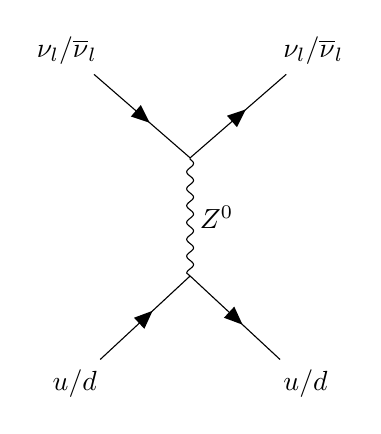
\begin{tikzpicture}
	\begin{feynman}
	\vertex (a);
	\vertex [below=of a] (b);
	\vertex [above left=of a] (c) {\(\nu_{l} / \overline \nu_{l}\)};
	\vertex [above right=of a] (d) {\(\nu_{l} / \overline \nu_{l}\)};
	\vertex [below left=of b] (e) {\(u/d\)};
	\vertex [below right=of b] (f) {\(u/d\)};
	\diagram* {
		(c) -- [fermion] (a),
		(a) -- [fermion] (d),
		(e) -- [fermion] (b),
		(b) -- [fermion] (f),
		(a) -- [boson, edge label=\(Z^0\)] (b),
	};
	\end{feynman}
	\end{tikzpicture}
	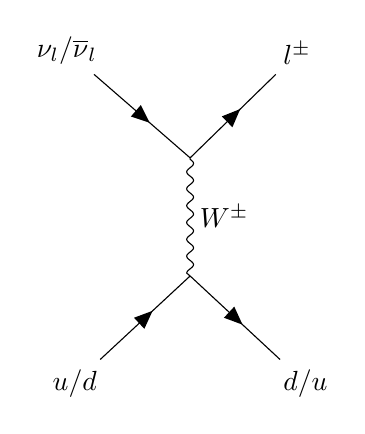
\begin{tikzpicture}
	\begin{feynman}
	\vertex (a);
	\vertex [below=of a] (b);
	\vertex [above left=of a] (c) {\(\nu_{l} / \overline \nu_{l}\)};
	\vertex [above right=of a] (d) {\(l^\pm\)};
	\vertex [below left=of b] (e) {\(u/d\)};
	\vertex [below right=of b] (f) {\(d/u\)};
	\diagram* {
		(c) -- [fermion] (a),
		(a) -- [fermion] (d),
		(e) -- [fermion] (b),
		(b) -- [fermion] (f),
		(a) -- [boson, edge label=\(W^\pm\)] (b),
	};
	\end{feynman}
	\end{tikzpicture}
	\caption{The neutrino deep inelastic scattering processes NC (left) and CC (right) in matter is shown in the figure above for interactions with nucleon component quarks.
	In both cases, significant momentum can be imparted to the outgoing quark which will result in the production of a hadronic particle cascade.
	In NC interactions, only the hadronic cascade may be detectable as the interaction product is a neutrino which is unlikely to undergo another interaction within the detection medium.
	Interactions of the CC variety on the other hand, produce a charged lepton in addition to the hadronic cascade.
	This charged lepton can also be detected if it receives enough energy.}
	\label{fig:DIS}
\end{figure}

\begin{figure}
\begin{tikzpicture}
\begin{feynman}
\vertex (a);
\vertex [right=of a] (b);
\vertex [above left=of a] (c) {\(\overline \nu_{e}\)};
\vertex [below left=of a] (d) {\(e^-\)};
\diagram* {
	(c) -- [fermion] (a),
	(a) -- [fermion] (d),
	(a) -- [boson, edge label=\(W^+\)] (b),
};
\end{feynman}
\end{tikzpicture}
\caption{}
\label{}
\end{figure}


\textbf{What are the products from neutrino interactions that allow us to detect neutrinos?}

\textbf{What is the process by which we detect these products in existing detectors?}


\section{The IceCube detector}

\begingroup
\graphicspath{{results/HESE_Final_Paper/}}
\subfile{results/HESE_Final_Paper/sections/detectorselection/detector}
\endgroup

\chapter{Searching for astrophysical neutrinos: High Energy Starting Events}

\section{Event selection\label{sec:selection}}
\begingroup
\graphicspath{{results/HESE_Final_Paper/}}
\chapter{Searching for astrophysical neutrinos: High Energy Starting Events}

\section{Event selection\label{sec:selection}}
\begingroup
\graphicspath{{results/HESE_Final_Paper/}}
\chapter{Searching for astrophysical neutrinos: High Energy Starting Events}

\section{Event selection\label{sec:selection}}
\begingroup
\graphicspath{{results/HESE_Final_Paper/}}
\input{results/HESE_Final_Paper/sections/detectorselection/selection}
\endgroup

\section{Determination of atmospheric neutrino and muon backgrounds\label{sec:backgrounds}}
\begingroup
\graphicspath{{results/HESE_Final_Paper/}}
\input{results/HESE_Final_Paper/sections/backgrounds}
\endgroup

\section{Accounting for veto effects}
\endgroup

\section{Determination of atmospheric neutrino and muon backgrounds\label{sec:backgrounds}}
\begingroup
\graphicspath{{results/HESE_Final_Paper/}}
\chapter{Determination of atmospheric neutrino and muon backgrounds}

\section{Cosmic rays}

\section{Neutrino production in air-showers}

\section{Accounting for veto effects}

\section{Muon backgrounds}

\endgroup

\section{Accounting for veto effects}
\endgroup

\section{Determination of atmospheric neutrino and muon backgrounds\label{sec:backgrounds}}
\begingroup
\graphicspath{{results/HESE_Final_Paper/}}
\chapter{Determination of atmospheric neutrino and muon backgrounds}

\section{Cosmic rays}

\section{Neutrino production in air-showers}

\section{Accounting for veto effects}

\section{Muon backgrounds}

\endgroup

\section{Accounting for veto effects}
\chapter{Event reconstruction and simulation}\label{chapter:reconstruction}
\begingroup
\graphicspath{{results/HESE_Final_Paper/}}
\chapter{Event reconstruction and simulation}\label{chapter:reconstruction}
\begingroup
\graphicspath{{results/HESE_Final_Paper/}}
\chapter{Event reconstruction and simulation}\label{chapter:reconstruction}
\begingroup
\graphicspath{{results/HESE_Final_Paper/}}
\input{results/HESE_Final_Paper/sections/reconstruction}
\endgroup
\endgroup
\endgroup
\chapter{Determination of atmospheric neutrino and muon backgrounds}

\section{Cosmic rays}

\section{Neutrino production in air-showers}

\section{Accounting for veto effects}

\section{Muon backgrounds}

\chapter{Dealing with limited simulation samples}


\chapter{Analysis}\label{chapter:analysis}

The goal of the analysis in this chapter is to characterize the astrophysical neutrino spectrum using a high-purity sample of events.
On its own, this may not provide the great insight that we desire into larger problems of astropysical neutrino origin or cosmic ray acceleration mechanisms.
However, the detailed measurements performed here are a vital piece of the puzzle that may help us to answer these larger questions in the long run.
In pursuit of these measurements a handful of new techniques were also developed, and these will certainly improve the other measurements we make going forward.
This chapter combines the analysis components outlined in previous chapters with different definitions of the astrophysical neutrino flux and applies the statistical inference techniques of \refsec{sec:statistics} to the analysis structure of \reffig{fig:analysis_overview}.
With this a wide variety of tests and measurements of the astrophysical flux are explored and their results examined.

\section{Characterization of the astrophysical neutrino flux\label{sec:diffuse}}
\begingroup
\graphicspath{{results/HESE_Final_Paper/}}
\input{results/HESE_Final_Paper/sections/diffuse/diffuse}
\endgroup

\subsection{Generic models\label{sec:generic_models}}
\begingroup
\graphicspath{{results/HESE_Final_Paper/}}
\input{results/HESE_Final_Paper/sections/diffuse/generic_models}
\endgroup

\subsubsection{Single power-law flux\label{sec:spl}}
\begingroup
\graphicspath{{results/HESE_Final_Paper/}}
\input{results/HESE_Final_Paper/sections/diffuse/spl}
\endgroup

\subsubsection{Double power-law flux\label{sec:dpl}}
\begingroup
\graphicspath{{results/HESE_Final_Paper/}}
\input{results/HESE_Final_Paper/sections/diffuse/dpl}
\endgroup

\subsubsection{Single power law with spectral cutoff\label{sec:cutoff}}
\begingroup
\graphicspath{{results/HESE_Final_Paper/}}
\input{results/HESE_Final_Paper/sections/diffuse/cutoff}
\endgroup

\subsubsection{Log-parabola flux\label{sec:log_parabola}}
\begingroup
\graphicspath{{results/HESE_Final_Paper/}}
\input{results/HESE_Final_Paper/sections/diffuse/lppl}
\endgroup

\subsubsection{Segmented power-law flux\label{sec:unfolding}}
\begingroup
\graphicspath{{results/HESE_Final_Paper/}}
\input{results/HESE_Final_Paper/sections/diffuse/segmented}
\endgroup

\subsection{Atmospheric flux from charmed hadrons\label{sec:prompt}}
\begingroup
\graphicspath{{results/HESE_Final_Paper/}}
\input{results/HESE_Final_Paper/sections/diffuse/prompt}
\endgroup

\subsection{Source-specific models\label{sec:specific_models}}
\begingroup
\graphicspath{{results/HESE_Final_Paper/}}
\input{results/HESE_Final_Paper/sections/diffuse/specific_models}
\endgroup
\chapter{Conclusions and next steps\label{chapter:conclusions}}
\section{Analysis conclusions\label{sec:analysis_conclusions}}
\begingroup
\graphicspath{{results/HESE_Final_Paper/}}
\chapter{Conclusions and next steps\label{chapter:conclusions}}
\section{Analysis conclusions\label{sec:analysis_conclusions}}
\begingroup
\graphicspath{{results/HESE_Final_Paper/}}
\chapter{Conclusions and next steps\label{chapter:conclusions}}
\section{Analysis conclusions\label{sec:analysis_conclusions}}
\begingroup
\graphicspath{{results/HESE_Final_Paper/}}
\input{results/HESE_Final_Paper/sections/conclusions}
\endgroup
\FloatBarrier

\section{Next steps}
The analysis presented here updated previous studies of the HESE sample, and is only a small part of the picture for astophysical neutrinos and the mystery of cosmic ray origin.
However, the techniques and solutions developed here remain broadly applicable to future analyses, and will enable more precise measurements as more data is accumulated and additional samples are developed.

From the perspective of analyzing the astrophysical neutrino flux...
\endgroup
\FloatBarrier

\section{Next steps}
The analysis presented here updated previous studies of the HESE sample, and is only a small part of the picture for astophysical neutrinos and the mystery of cosmic ray origin.
However, the techniques and solutions developed here remain broadly applicable to future analyses, and will enable more precise measurements as more data is accumulated and additional samples are developed.

From the perspective of analyzing the astrophysical neutrino flux...
\endgroup
\FloatBarrier

\section{Next steps}
The analysis presented here updated previous studies of the HESE sample, and is only a small part of the picture for astophysical neutrinos and the mystery of cosmic ray origin.
However, the techniques and solutions developed here remain broadly applicable to future analyses, and will enable more precise measurements as more data is accumulated and additional samples are developed.

From the perspective of analyzing the astrophysical neutrino flux...


%\bibliography{results/HESE_Final_Paper/hesebiblio,results/mcllh_paper/likelihood,results/passing_fractions_paper/nuveto,thesis-citations}


\chapter*[Bibliography]{Bibliography}
\addcontentsline{toc}{chapter}{Bibliography}
\printbibliography[heading=none]
\refstepcounter{chapter}

\clearpage
\newpage
\appendix

\begingroup
\graphicspath{{results/HESE_Final_Paper/}}
\chapter{HESE source searches}
\section{High-energy astrophysical neutrino source searches\label{sec:sources}}
\subfile{results/HESE_Final_Paper/sections/sources}
\section{Event comparison\label{sec:comparison}}
\subfile{results/HESE_Final_Paper/appendices/comparison}
\section{Source catalog\label{sec:source_catalog}}
\subfile{results/HESE_Final_Paper/appendices/sources_table}

\chapter{HESE diffuse flux measurements}
%\section{Expected number of events table\label{sec:events_table}}
%\subfile{results/HESE_Final_Paper/appendices/event_table}
%\section{Sideband distributions\label{sec:sidebands}}
%\subfile{results/HESE_Final_Paper/appendices/sidebands}
%\section{Effects of systematics in analysis distributions\label{sec:extendedsys}}
%\subfile{results/HESE_Final_Paper/appendices/extendedsys}
\section{Data release for additional characterization of the astrophysical neutrino flux\label{sec:release}}
\subfile{results/HESE_Final_Paper/appendices/release}
\endgroup

\end{document}
